% 2003 年粤桂卷第 16 题：5 个行政区域地图着色示意图
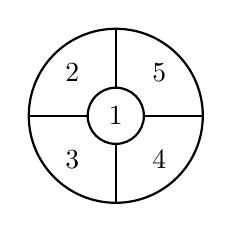
\begin{tikzpicture}[scale=0.85]
  \draw[thick] (0,0) circle (1.3);
  \draw[thick] (0,-1.3)--(0,1.3) (-1.3,0)--(1.3,0);
  \draw[thick,fill=white] (0,0) circle (0.42);
  \node at (0,0) {1};
  \node at (-0.65,0.65) {2};
  \node at (0.65,0.65) {5};
  \node at (-0.65,-0.65) {3};
  \node at (0.65,-0.65) {4};
\end{tikzpicture}
